% Adapted from
%  https://www.overleaf.com/latex/templates/pitt-state-physics-homework-template/wdsxknmntnxk

\documentclass[12pt]{article}
\usepackage[paper=letterpaper,margin=2cm]{geometry}
\usepackage{amsmath}
\usepackage{amssymb}
\usepackage{amsfonts}
\usepackage{newtxtext, newtxmath}
\usepackage{enumitem}
\usepackage{titling}
\usepackage{graphicx}
\usepackage[colorlinks=true]{hyperref}

\setlength{\droptitle}{-6em}

% Enter the specific assignment number and topic of that assignment below, and replace "Your Name" with your actual name.
\title{ENPM808W Homework \#1}
\author{Daniel M. Sahu}
\date{\today}

\begin{document}
\maketitle
\begin{enumerate}[leftmargin=\labelsep]
\item Analysis of simulated New York Times webpage activity.

  Problem \#1 involves loading and analyzing data which simulates page activity on the New York Times
  website over the course of a month. The simulated data includes user metadata like age, gender, etc.
  (if the user is logged in), as well as impressions (page views) and clicks.
  
  All code for Problem \#1 can be found on \href{https://github.com/danielmohansahu/data-science-exercises/tree/main/hw1}{GitHub}.
  See \href{https://github.com/danielmohansahu/data-science-exercises/blob/main/hw1/analyze_nyt.py}{this script} in particular.
  
  \textbf{Data Cleaning:}
  
  The data is contained in 31 CSV files, one for each date. Data cleaning was fairly straightforward - the only
  handling required was to avoid lumping metadata for logged in users with metadata for anonymous users, as certain
  field defaults cause misleading results. For example, the "gender" field for anonymous users defaults to $0$, which
  is the exact same value as female logged in users. To avoid this (and similar) issues we explicitly cast
  anonymous user data as UNKNOWN.

  \textbf{Parts (a,b):}
  
  After data cleaning our first goal was to plot the click-through-rate (CTR) for a variety of different age categories.
  Additionally, we wanted to split the data across other interesting categories to see what sort of trends presented
  themselves. Figures \ref{fig:p1_b_i} and \ref{fig:p1_b_iii} summarize our results.
  
  \begin{figure}[htb]
    \begin{center}
      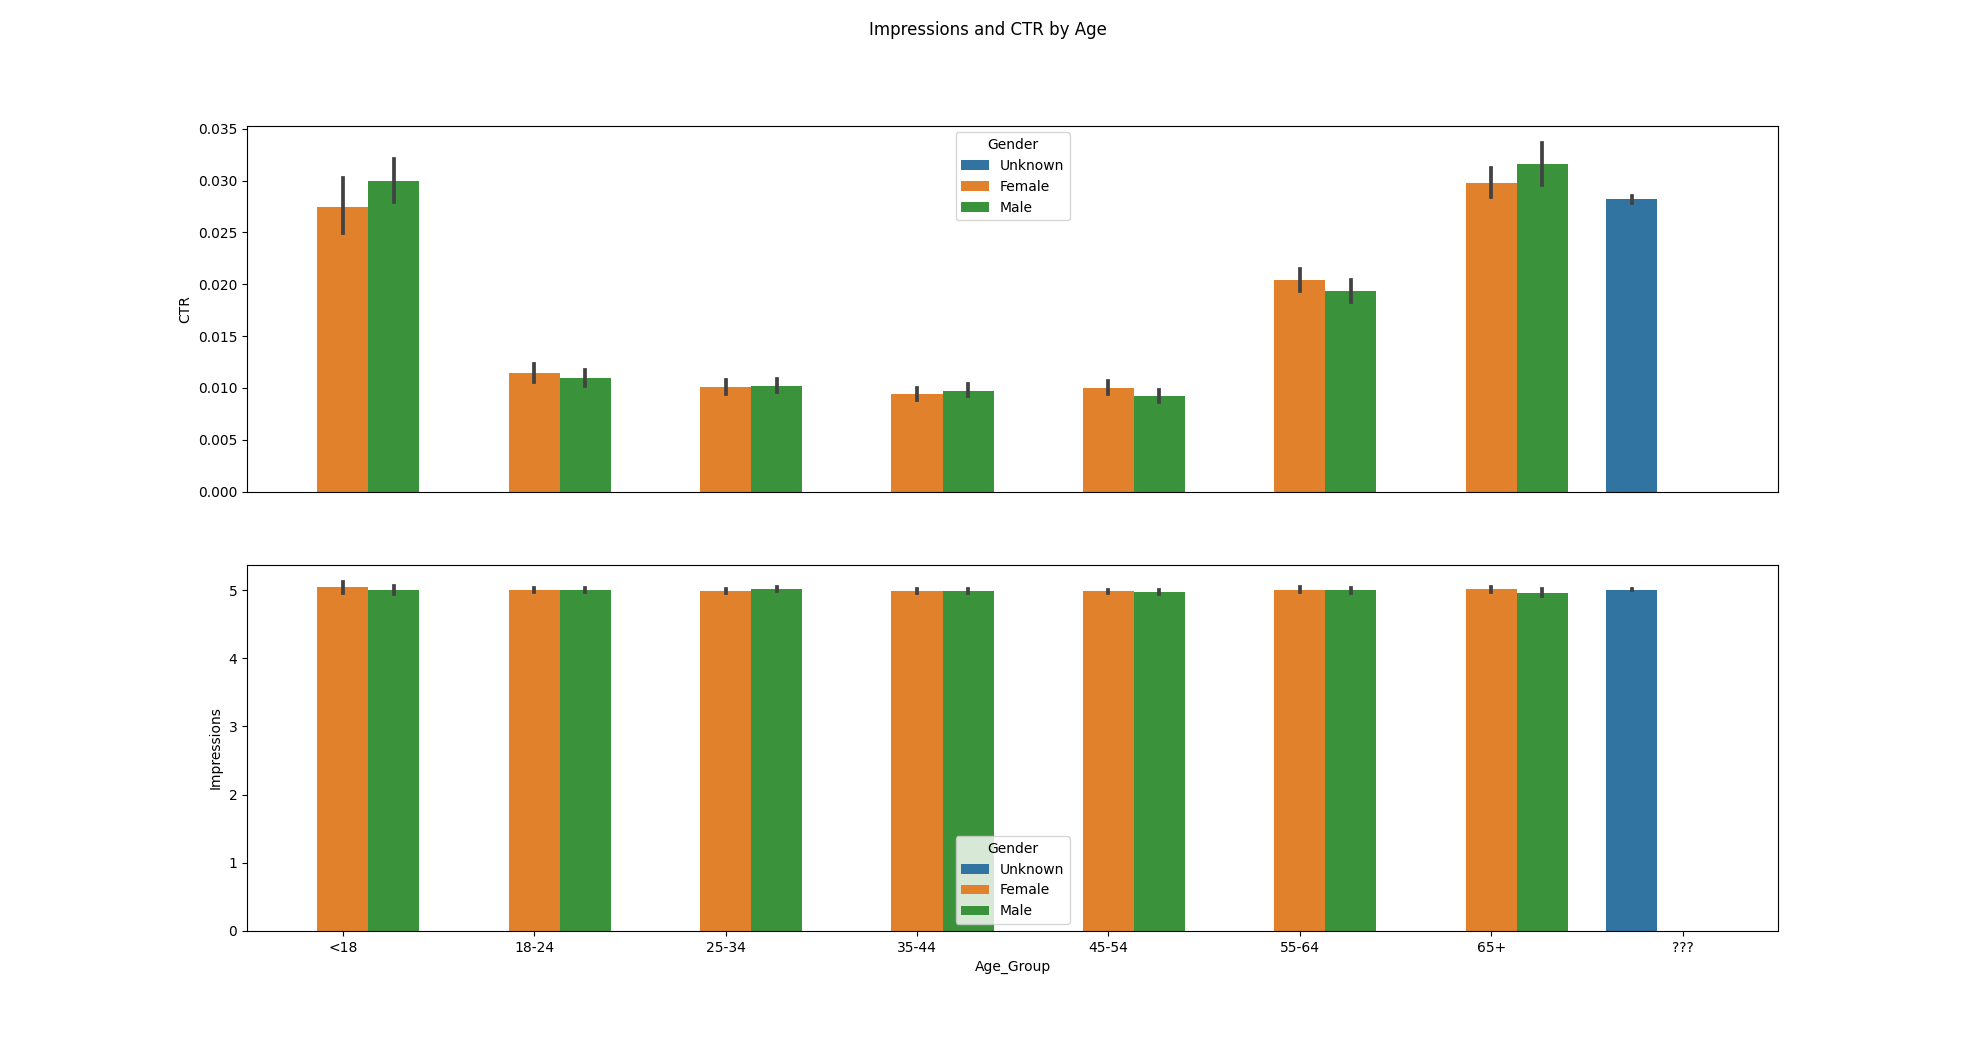
\includegraphics[width=\textwidth]{media/p1_b_i.png}
    \end{center}
    \caption{Impressions and CTR by Age}
    \label{fig:p1_b_i}
  \end{figure}
 
  \begin{figure}[htb]
    \begin{center}
      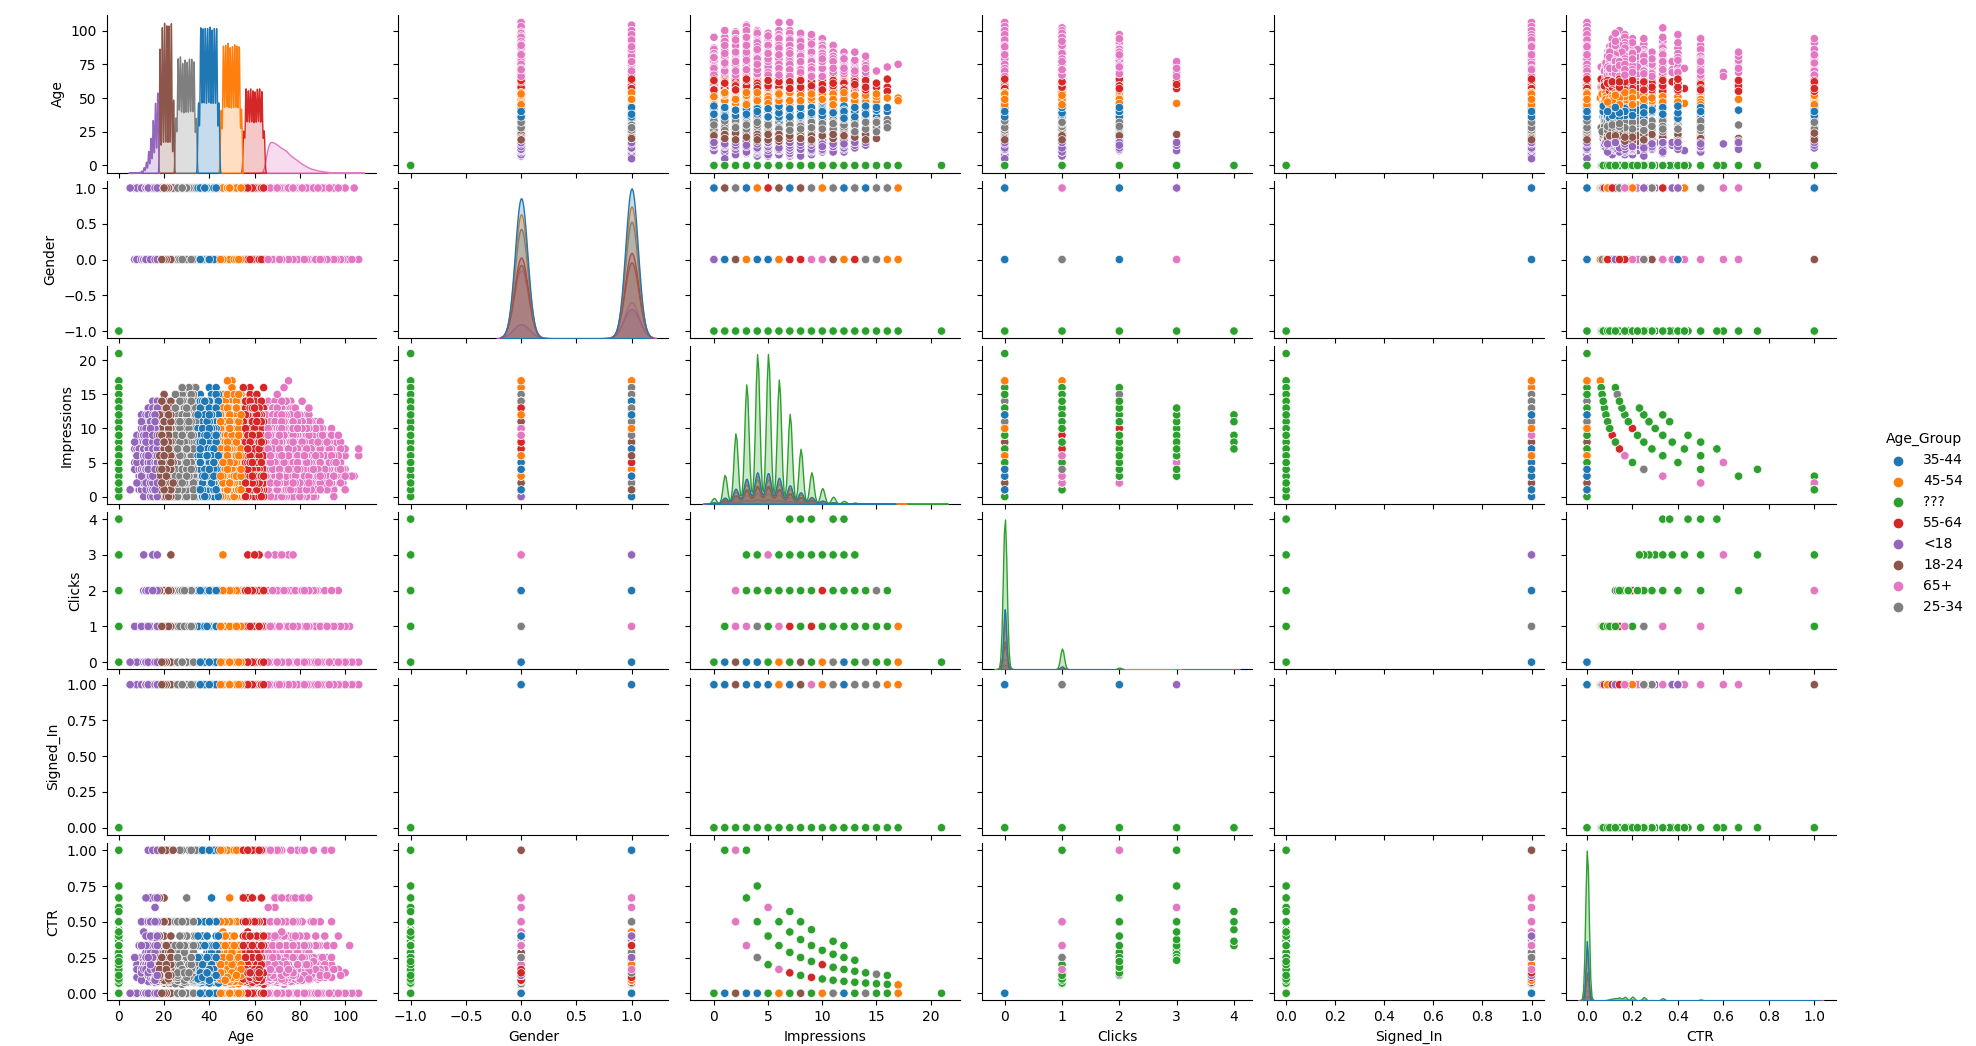
\includegraphics[width=\textwidth]{media/p1_b_iii.png}
    \end{center}
    \caption{Categorical Pairplot}
    \label{fig:p1_b_iii}
  \end{figure}

  Figure \ref{fig:p1_b_i} shows the Impressions and CTR of our various age groups. To handle anonymous users we deliberately
  split them out into a separate category. Each age group is also split along gender lines (except anonymous users, of course).
  Although the average number of Impressions is fairly stable for all users, we see a marked difference in CTR based on age
  group. There's a clear trend where younger ("<18") and older ("65+") users have relatively high CTRs. Users in the middle
  tend to click less for the same number of Impressions.

  The investigating of Figure Figure \ref{fig:p1_b_i} led to the conclusion that a more holistic view of the data would be useful.
  To that end we used the Python seaborn package's pairplot function to see if any other relationships stand out. Figure \ref{fig:p1_b_iii}
  shows the result. Although most of the pairwise relationships aren't interesting, there are a couple of notworth plots:
  \begin{itemize}
    \item The Histogram plot of Impressions vs. Impressions demonstrates that the majority of our users are \textit{not} logged in.
    \item The plots of Impressions vs. CTR show trend lines that clearly indicate that this is fake data. They look like this because
      the number of clicks are bounded by [0,4], which is much too clean for real-world data.
  \end{itemize}

  \textbf{Parts (c,d):}
  
  In Parts (a,b) the only interesting trend we noted was that there's a marked relationship between Age Group and CTR. All that analysis
  was done on a single day's data though, so the next step is to analyze trends over time. To that end we developed a number of metrics which
  summarize the overall information for a given date and compare those metrics over time.
  
  The metrics we settled upon are:
  \begin{itemize}
    \item Count: The number of users collected in a given day.
    \item CTR Mean: The mean of the CTR.
    \item CTR Stddev: The standard deviation of CTR.
    \item Clicks Mean: The mean of the clicks.
    \item Clicks Stddev: The standard deviation of Clicks.
    \item Impressions Mean: The mean of the impressions.
    \item Impressions Stddev: The standard deviation of impressions.
  \end{itemize}

  In addition to the above we also pass forward the following metadata for ease of analysis:

  \begin{itemize}
    \item Day: The day of the month this data comes from.
    \item Age Group: Metrics are collected per-age group for a given day, not collectively.
  \end{itemize}
  
  \begin{figure}[htb]
    \begin{center}
      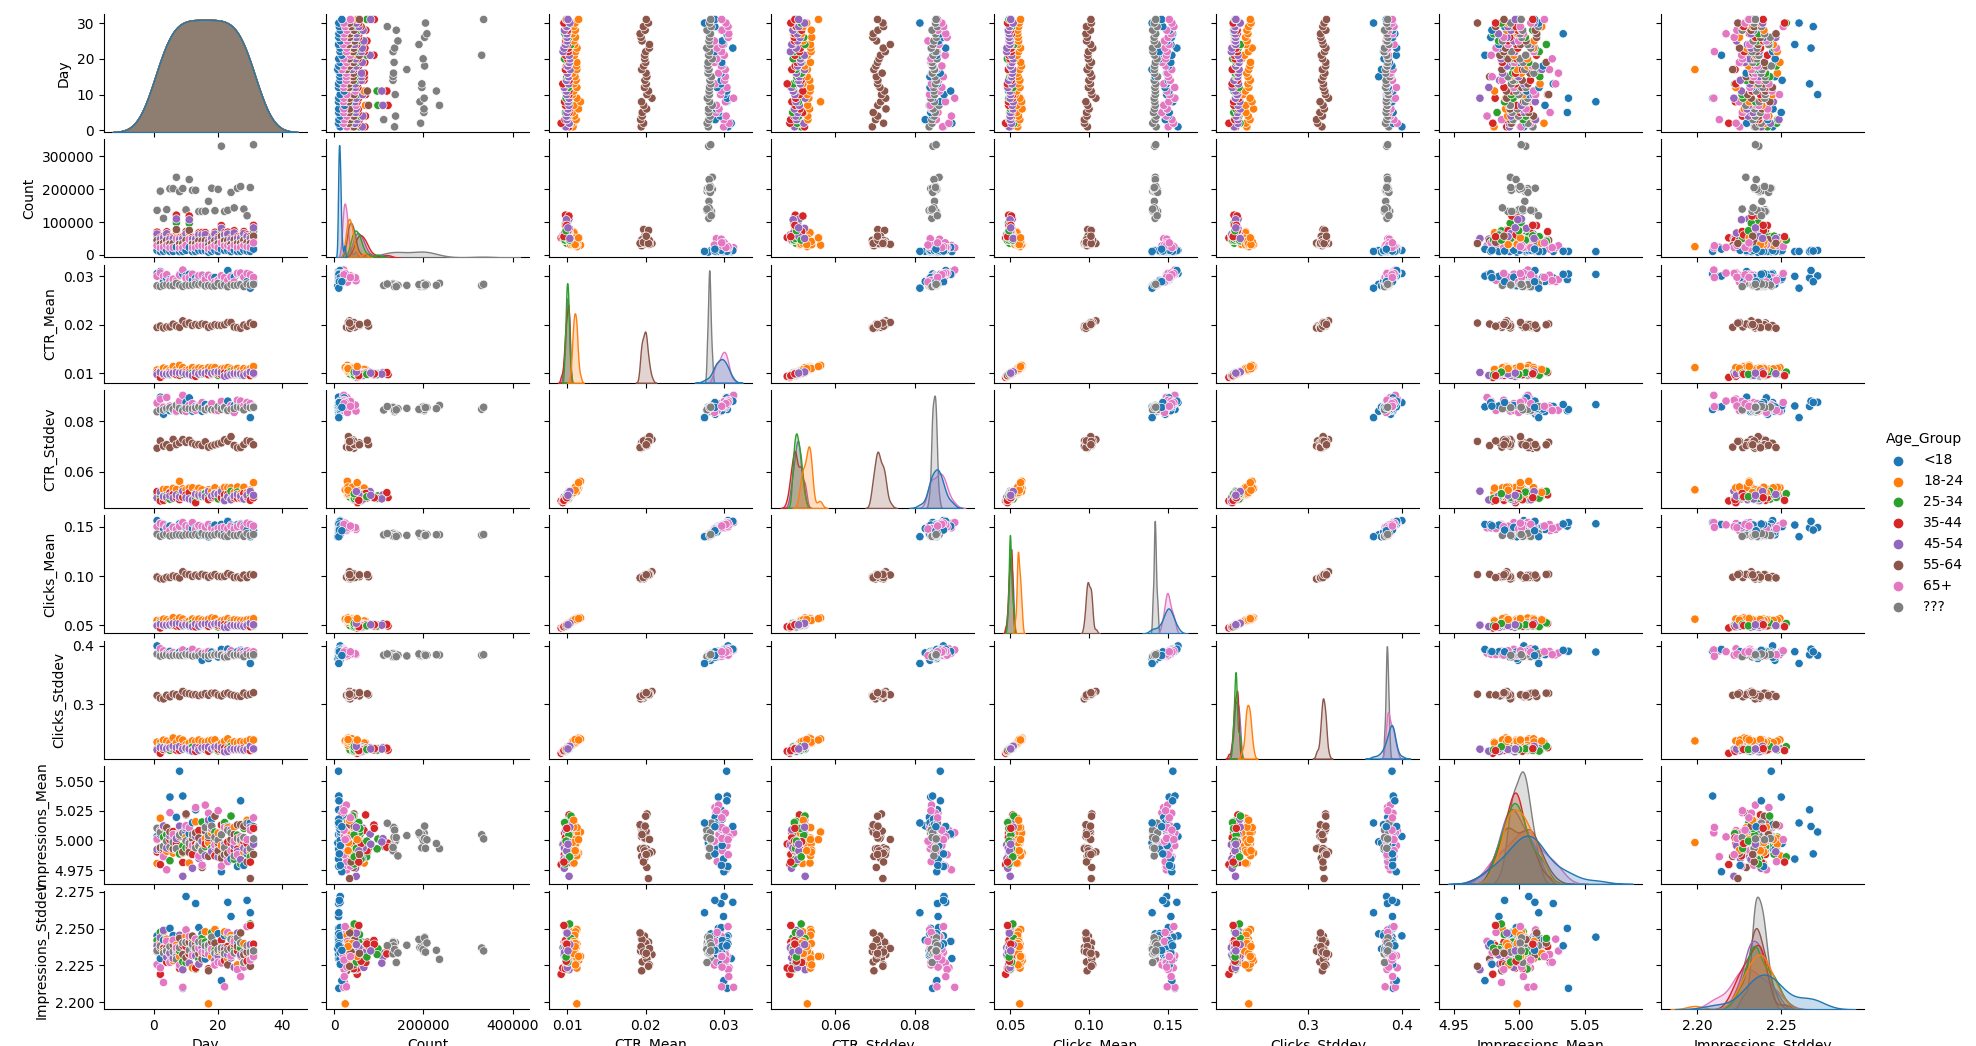
\includegraphics[width=\textwidth]{media/p1_c_i.png}
    \end{center}
    \caption{Metric Pairplot}
    \label{fig:p1_c_i}
  \end{figure}
  
  Our metric information across time is summarized in another pairplot in Figure \ref{fig:p1_c_i}. Although this plot
  can be somewhat overwhelming, it gives a high enough snapshot to allow us to spot a few interesting trends:
  \begin{itemize}
    \item Although there's no clear temporal trend like "CTR increases over time" it is clear that all the days are not
      homogeneous. There are a number of days which stand out as "fast news days" where the user count is significantly
      higher than average. See the "Day vs. Count" plot.
    \item Although there's no clear trend for number of Impressions, the same marked relationship between Age Group and
      CTR / Clicks is present over time.
  \end{itemize}
  
  The trend between Age Group and Clicks / CTR is so strong that we can visually infer that the data was simulated with
  (very roughly) the following Gaussian distributions:
  
  \begin{center}
    \begin{tabular}{l*{7}{c}r}
      Metric          & <18 & 18-24 & 25-34 & 35-44 & 45-54 & 55-64 & 65+ & ??? \\
      \hline
      Clicks (mean)   & 0.15 & 0.05 & 0.05 & 0.05 & 0.05 & 0.10 & 0.15 & 0.15 \\
      Clicks (stddev) & 0.40 & 0.25 & 0.25 & 0.25 & 0.25 & 0.30 & 0.40 & 0.40 \\
      CTR (mean)      & 0.03 & 0.01 & 0.01 & 0.01 & 0.01 & 0.02 & 0.03 & 0.03 \\
      CTR (stddev)    & 0.90 & 0.05 & 0.05 & 0.05 & 0.05 & 0.07 & 0.90 & 0.90 \\
    \end{tabular}
  \end{center}      

\item Analysis of a self-selected dataset.
  
  The mandate of this problem was to find and analyze a non-trivial dataset. We chose to analyze
  \href{https://www.kaggle.com/datasets/ramjasmaurya/us-police-shootings-from-20152022}{data on police shootings in the U.S. from Kaggle}.
  This dataset includes select information about police shootings that resulted in fatalities between 2015 and 2022. The goal here
  was mainly to get a sense for \textit{what} information is actually available on such a controversial topic for my edification.
  
  As with Problem \#1 all the code used to generate plots is found on Github, specifically \href{https://github.com/danielmohansahu/data-science-exercises/blob/main/hw1/analyze_shootings.py}{this script}.

  \textbf{Raw Data Overview:}

  The raw dataset contains the following columns. Items marked "unused" were not used in further analysis, either due to resource constraints
  or because a use couldn't be determined.

  \begin{itemize}
    \item $id$ (unused): Unique identifier.
    \item $name$ (unused): The name of the deceased.
    \item $date$: The date of the encounter.
    \item $manner of death$ (unused): How the deceased was killed.
    \item $armed$: Weapon the deceased had (if any).
    \item $age$: The age of the deceased.
    \item $gender$: The gender of the deceased.
    \item $race$: The race of the deceased.
    \item $city$ (unused): The city in which the encounter occurred.
    \item $state$: The state in which the encounter occurred.
    \item $signs$ of mental illness (unused): Whether or not the deceased exhibited signs of mental illness.
    \item $threat level$ (unused): Perceived threat level of the deceased.
    \item $flee$: The means of attempted escape, if applicable.
    \item $body camera$ (unused): Whether or not the officer(s) were wearing a body camera.
    \item $longitude$ (unused): Longitude of the incident.
    \item $latitude$ (unused): Latitude of the incident.
    \item $is geocoding exact$ (unused): Whether or not the coordinates are exact.
  \end{itemize}

  \textbf{Data Munging:}

  Much of the raw information presented above was desired, but some of it wasn't immediately useful in its present form.
  To that end the following operations were performed to extract salient information:
  \begin{enumerate}
    \item $date$, $age$, $gender$ were used directly.
    \item $race$ was used directly, with NaNs replaced by $O$ (Other).
    \item $year$ was extracted from $date$.
    \item $region$ was extracted by assigning $state$ information to the corresponding geographic region (e.g. SOUTHWEST).
    \item $weapon$ was extracted by binning $armed$ into $GUN$, $OTHER$, $UNARMED$ as a rough proxy of dangerousness.
    \item $armed$ was converted to a boolean.
    \item $escaping$ was extracted by converting $flee$ to a boolean.
    \item All NaNs found after the above were dropped.
  \end{enumerate}

  \textbf{Cleaned Data Overview:}

  \begin{figure}[htb]
    \begin{center}
      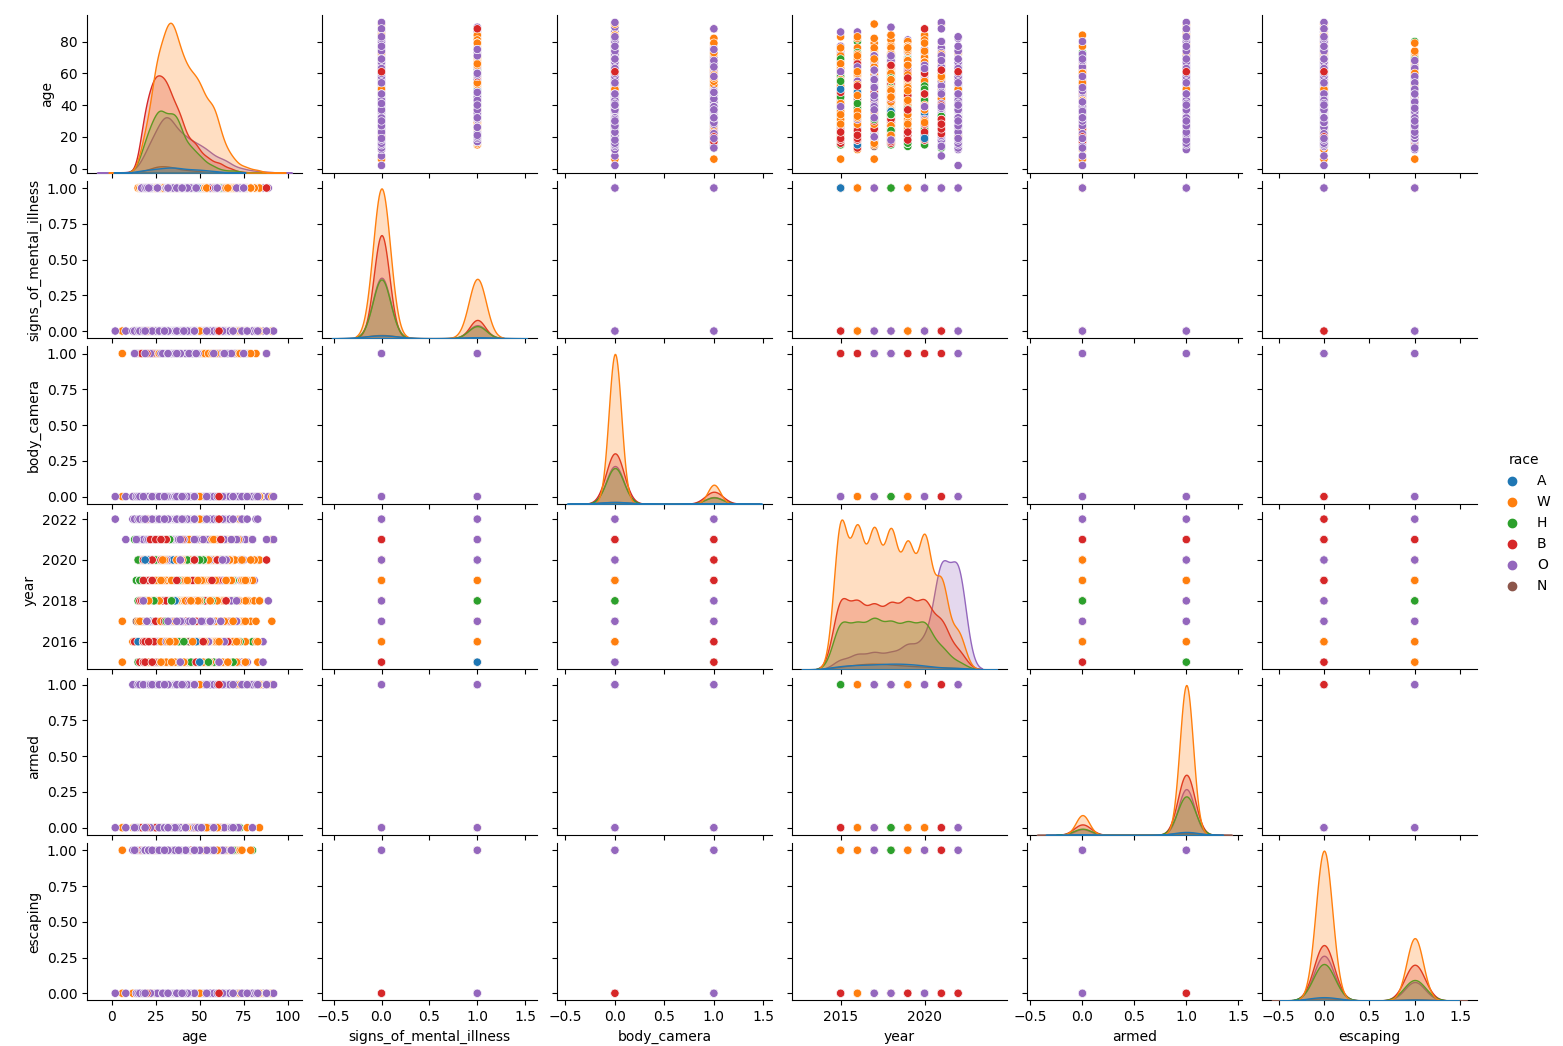
\includegraphics[width=\textwidth]{media/p2_pairplot.png}
    \end{center}
    \caption{Cleaned Data Pairplot}
    \label{fig:p2_pairplot}
  \end{figure}
  
  \textbf{Temporal Trend Analysis:}

  \begin{figure}[htb]
    \begin{center}
      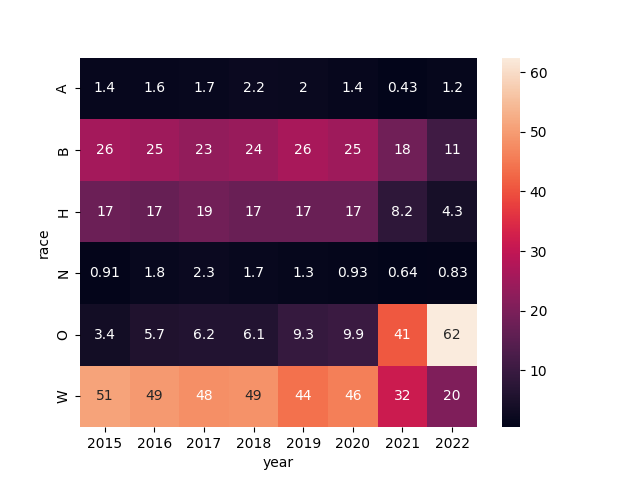
\includegraphics[width=\textwidth]{media/Count_by_Race_over_Time.png}
    \end{center}
    \caption{Count by Race over Time}
    \label{fig:p2_count_by_race_time}
  \end{figure}

  \begin{figure}[htb]
    \begin{center}
      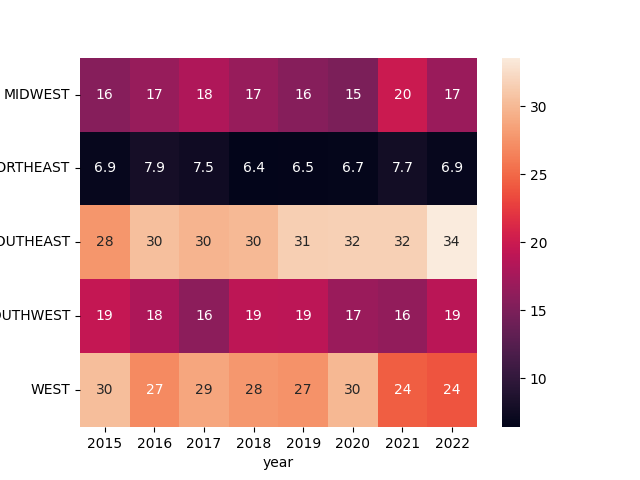
\includegraphics[width=\textwidth]{media/Count_by_Region_over_Time.png}
    \end{center}
    \caption{Count by Region over Time}
    \label{fig:p2_count_by_region_time}
  \end{figure}

  \begin{figure}[htb]
    \begin{center}
      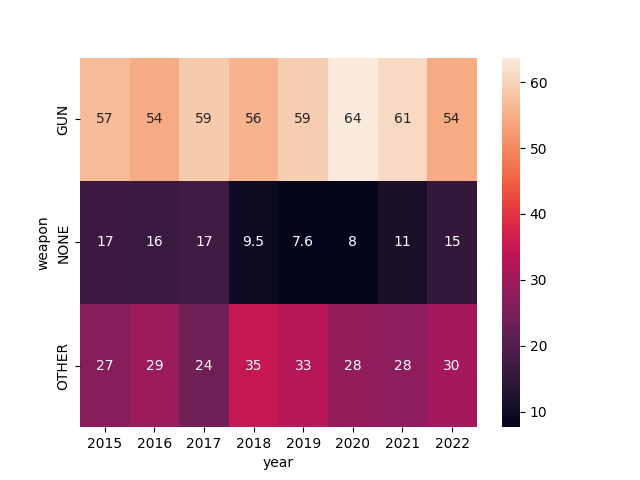
\includegraphics[width=\textwidth]{media/Count_by_Weapon_over_Time.png}
    \end{center}
    \caption{Count by Weapon over Time}
    \label{fig:p2_count_by_weapon_time}
  \end{figure}
  
  \textbf{Other Analyses:}

  \begin{figure}[htb]
    \begin{center}
      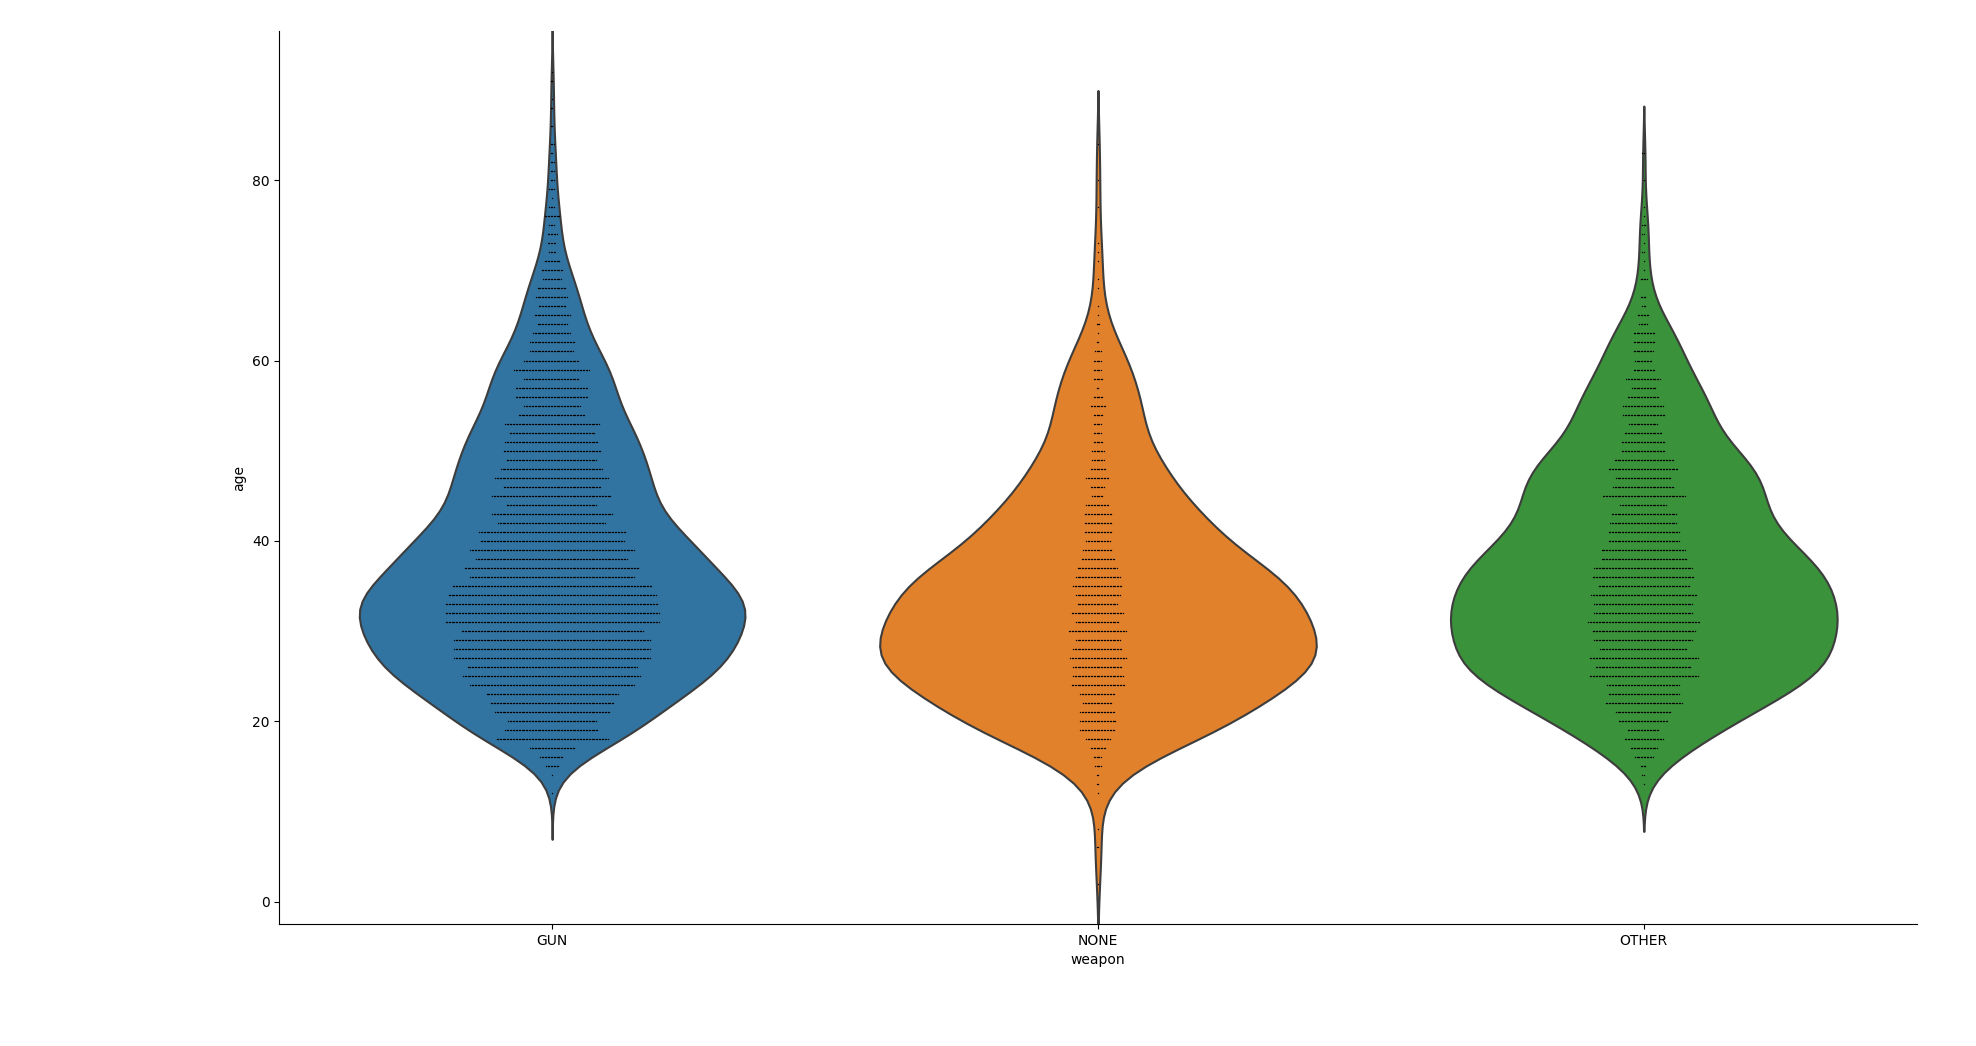
\includegraphics[width=\textwidth]{media/p2_age_vs_weapon.png}
    \end{center}
    \caption{Age vs. Weapon}
    \label{fig:p2_age_vs_weapon}
  \end{figure}
  
  \textbf{Interpretation / Interesting Notes:}
  
\end{enumerate}
\end{document}